% !TeX root = RJwrapper.tex
\title{MTBrush: Linked Histogram Brushing for Exploration of Multiple
Hypotheses}
\author{by Yixing Tu, Marc Chevrette, Chris Thomas, Jo Handelsman, and Kris
Sankaran}

\maketitle

\abstract{%
MTBrush is an R package for testing and exploring a large collection of
hypothesis. By applying the principle of dynamic linking to the multiple
hypothesis testing setting, the package supports efficient navigation of
estimated effects and their relationships. The package is motivated by
problems that require estimation of an ensemble of \(n\) linear models,
where each model is associated with one feature --- for example, a gene
or metabolite. MTBrush provides an interactive interface based on
brushing dynamically linked histograms. By comparing the highlighted
intervals across histograms of different statistics and by
cross-referencing with scatterplots of the original data, users can
rapidly evaluate visual queries across an ensemble of models. We apply
the MTBrush to two applications in microbiome and spatial data analysis,
respectively. We find that MTBrush can help users easily identify
interaction effects in multiple hypothesis testing with complex designs.
}

\hypertarget{keywords}{%
\section{Keywords}\label{keywords}}

Multiple hypothesis testing, interactive visualization, dynamic linking,
interaction effects, R package

\hypertarget{introduction}{%
\section{Introduction}\label{introduction}}

Large-scale datasets often emerge by combining many smaller, parallel
ones. For example, in microbiome studies, it is common to simultaneously
measure the abundances of thousands of species, and each species can be
considered as its own, small-scale context. When our goal is to sift
through this collection in search for interesting associations (e.g.,
with a treatment), it is common to compute one summary statistic per
feature and use these summaries to focus subsequent attention. This is
the logic behind multiple hypothesis testing. Typically, the results of
multiple hypothesis tests are printed as tables of significant features,
and studies often report these as targets for potential follow-up. While
these lists are useful, it is often necessary to more deeply explore
properties of the flagged hypotheses in order to develop more
substantive interpretations and design further experiments. For example,
it is valuable to know whether several flagged metabolites belong to the
same metabolic pathway.

To support these more complete interpretations, we develop the MTBrush
package. The package provides an interactive Shiny interface to the
results of a collection of separate, but related, multiple hypothesis
tests. The interface builds from the methodological proposals of
\citep[\citet{stephens}]{efron2021computer}, where the histogram of test
statistics serves as a device for estimating false discovery rates.
While we similarly focus on the empirical distribution of test
statistics, MTBrush places these histograms in a central role, allowing
users to directly inspect these histograms within context. An advantage
of this perspective is that it becomes possible to explore relations in
more complex designs, including those where formal false discovery rate
estimation procedures may be unavailable. For example, in Case Study 1
below, we are interested in evaluating metabolome-wide differential
expression under multiple perturbations to a model microbial system.
Interest lies in the possibility of the emergence of synergies when
applying multiple perturbations simultaneously. On their own, each
perturbation leads to a multiple hypothesis testing problem. Viewed
together, the collection of perturbations leads to an ensemble of
related multiple testing problems. Which metabolites are significantly
differentially expressed across multiple perturbations? To what extent
are the differentially expressed metabolites shared across perturbation
types? MTBrush provides as a natural exploratory framework for such
comparisons.

One of the difficulties of visualization in the multiple testing setting
is that the data of interest are inherently high-dimensional, and static
visualization is limited in the number of dimensions that it can
naturally encode \citep{Wills}. That is, though it is straightforward to
visualize distributional differences across conditions for each feature
(e.g., through a set of boxplots), when the number of features grows,
such an approach becomes untenable. In the high-dimensional
visualization literature, dynamic linking provides a strategy for
providing details on units of interest while maintaining global context
\color{violet} Add reference to Buja, Cook, Swayne (1996?) high
dimensional visualization \color{black}. Specifically, in dynamically
linked brushing, several views of a single underlying dataset are
presented simultaneously. When a user selects a subset of units in one
view, the corresponding units across all views are highlighted. In this
way, the user can build intuition about the distribution of feature
values across all panels, conditional on lying within the selected
subset for one panel. For example, linked scatterplot brushing can show
how groups of \(\geq 3\) features co-vary --- points lying in one region
for one scatterplot may consistently lie in a narrow region of a linked
scatterplot \color{violet} Add reference to Becker and Cleveland
scatterplot brushing \color{black}.

The remainder of the paper is structured as follows. Section 1 describes
the design of the MTBrush package, the inputs and outputs of the
available functions, and the practical workflow from testing to
interpretation. Section 2 provides two case studies, the first to
metabolomic analysis of a model microbiological system and the second to
a spatial analysis of home prices. We conclude with a brief summary.

\hypertarget{methods}{%
\section{Methods}\label{methods}}

MTBrush has two main types of functions: Helpers that support testing of
multiple hypotheses (Section 2.1) and methods for launching interactive
interfaces based on test results (Section 2.2).

\hypertarget{helper-functions-for-multiple-testing}{%
\subsection{Helper functions for multiple
testing}\label{helper-functions-for-multiple-testing}}

MTBrush provides utilities to apply multiple hypothesis testing across
features. We place special emphasis on situations where multiple test
statistics are generated for each feature, since when there are multiple
histograms of test statistics to compare, linked brushing is especially
helpful. Two functions support this step, \texttt{split\_dataset()} and
\texttt{fit\_statistics()}. The first function splits a dataset across
the features over which tests should be computed. For example, in the
metabolomic application below, this is used to split a single data.frame
across metabolites into a list of data.frames, one for each metabolite.
The second maps a user-specified hypothesis testing function across
features defined by the first. A description of the inputs and outputs
of this function are provided in Table 1.

\color{violet}

Can you figure out how to put the information below into the table
above? My guess is that the R Journal template file discusses how to
include / format tables for publication, but let me know if this is not
easy to find. \color{black}

\begin{Schunk}
\begin{table}

\caption{\label{tab:unnamed-chunk-2}Helper Methods}
\centering
\begin{tabu} to \linewidth {>{\raggedright}X>{\raggedright}X>{\raggedright}X>{\raggedright}X}
\hline
Function & Description & Inputs & Outputs\\
\hline
split\_dataset(df, group) & This function splits the given data set into many smaller subsets based on the feature of interest. Each subset only contains measurements of a sample and all subsets take same measurements. & `df`: A long `data.frame` with sample measurements across all features. `group`: The column name of the feature over which to split the `data.frame` for downstream testing. & A list with one `data.frame` for each feature specified in `group`.\\
\hline
fit\_statistics(subsets, lm\_func, group) & This method maps overall all groups of subsets and returns a set of test statistics associated with each. The testing function can be specified by the user. & `subsets`: List of `data.frame` subsets as output by `split\_dataset` `lm\_func`: A function that takes one subset of samples and returns a vector of test statistics associated with it. `group`: The name of the column used when initially splitting measurements across features. & A single `data.frame` with statistics from the collection of tests across features\\
\hline
\end{tabu}
\end{table}

\end{Schunk}

For example, we split a randomly generated dataset in the block below.
The simulated data supposes a design in which two perturbations (A and
B) are applied to 10 features of interest. For each combination of
perturbations, five samples are collected per feature. We annotate each
configuration of perturbations in two ways -- one column labeling which
perturbations are active (\texttt{condition}) and several providing a
binary encoding of the same conditions (\texttt{A} and \texttt{B}). The
\texttt{condition} column allows the user to customize the labeling of
perturbations in downstream visualization.

A linear model is then used to evaluate the existence of main and
interaction effects across the perturbations, for each feature of
interest. The \texttt{estimate} column in the output below includes
\(t\)-statistics associated with each term in the model. For each
feature, the empirical distribution of the \texttt{estimate} column is
approximately \(t\)-distributed, because in this simulated example,
there are no true significant effects. Finally, note the use of
nonstandard evaluation in both functions -- the \texttt{feature} column
is understood directly without quoting. This provides an interface
familiar from packages in the tidyverse.

\color{violet}

\begin{itemize}
\tightlist
\item
  This is a simple randomly generated dataset which doesn't have any
  non-null main or interaction effects. Could we create a version which
  does, and then include that in the package?
\item
  Is there a way to provide a default value for the \texttt{condition}
  column for \texttt{brush\_plots\_binary}? Having to include this makes
  the package a bit harder to use. At the very least, we should make
  sure that the ``condition'' column is described in the documentation
  for this function.
\end{itemize}

\begin{Schunk}
\begin{Sinput}
library(MTBrush)
library(tidyverse)

alpha = 2.6
beta1 = 0.3
beta2 = -0.5
beta3 = -1.3

error <- rnorm(20000, 0, 1)

example_data <- expand.grid(
  sample = seq_len(5),
  feature = seq_len(1000),
  X1 = c(FALSE, TRUE),
  X2 = c(FALSE, TRUE)
) %>%
  mutate(
    value = alpha + beta1*X1 + beta2*X2 + beta3*X1*X2 + error,
    condition = case_when( 
      X1 & X2 ~ "X1X2",
      X1 & !X2 ~ "X1",
      !X1 & X2 ~ "X2",
      !X1 & !X2 ~ "Neither"
      )
    )

fit_results <- example_data %>%
  split_dataset(feature) %>%
  fit_statistics(~ lm(value ~ X1 * X2, .), feature)
head(fit_results)
\end{Sinput}
\begin{Soutput}
#> # A tibble: 6 x 6
#>   feature term          estimate std.error statistic    p.value
#>   <chr>   <chr>            <dbl>     <dbl>     <dbl>      <dbl>
#> 1 1       (Intercept)     2.71       0.377     7.19  0.00000216
#> 2 1       X1TRUE          0.0605     0.533     0.113 0.911     
#> 3 1       X2TRUE         -0.669      0.533    -1.25  0.228     
#> 4 1       X1TRUE:X2TRUE  -1.55       0.754    -2.06  0.0562    
#> 5 2       (Intercept)     2.45       0.419     5.86  0.0000243 
#> 6 2       X1TRUE          0.167      0.592     0.281 0.782
\end{Soutput}
\end{Schunk}

\color{black}

\hypertarget{visualization-of-multiple-testing-results}{%
\subsection{Visualization of multiple testing
results}\label{visualization-of-multiple-testing-results}}

Given test statistic outputs associated with each feature, the next step
in the MTBrush workflow (Figure 1) is interactive visualization through
histogram brushing. Table 2 describes functions that implement this
step. Note that different functions are provided depending on whether
the perturbations are binary (active / inactive) or continuous --- we
focus discussion here on the binary case, but both settings are
illustrated in the case studies below.

An example initial view provided by these functions is given in Figure
\ref{fig:interface1}. This initial view includes several histograms of
test statistics (section A) and a scatterplot of original measurements
across all conditions (section B). Recall that several model terms may
be estimated for each feature, each associated with its own test
statistic. Each panel in (section A) corresponds to one model term.
Features with extreme values of a given test statistic appear in the
tails of the corresponding histogram. For example, based on the design
of the linear model input to \texttt{fit\_statistics}, features in the
right tail of panel \texttt{X1} in section A have systematically larger
values in the \texttt{X2} column of section B.

\color{violet} Can you place the functions below into a table, just like
for the statistical wrapper functions? Also,
\texttt{brush\_plots\_other} doesn't seem like a good name. Can you
rename it to something less vague? How about
\texttt{brush\_plots\_nonbi} \color{black}

\begin{Schunk}
\begin{table}

\caption{\label{tab:unnamed-chunk-4}Visualization Methods on Test Results}
\centering
\begin{tabu} to \linewidth {>{\raggedright}X>{\raggedright}X>{\raggedright}X>{\raggedright}X}
\hline
Function & Description & Inputs & Outputs\\
\hline
draw\_stats\_histogram( stats\_df) & This function generates histograms of statistics for all terms calculated by `fit\_statistics` which also serve as base plots in the Shiny App interface to make interactions on & `stats\_df`: A `data.frame` contains statistics of tests across features; the output from `fit\_statistics(subsets, lm\_func, group)` function & Histograms of statistics based on results from previous hypothesis testings across features\\
\hline
brush\_plots\_binary(df, stats\_df, group\_list, group, value) & This method launchs the Shiny app to show results from previous multiple hypothesis testings and allow users to query for details on conspicuous features. Use this function when the condition/explanatory variables have binary data type. & `df`: The same long `data.frame` with sample measurements across all features used in helper methods. `stats\_df`: A `data.frame` contains statistics of tests across features. `group\_list`: The list of distinct features after splitting the `data.frame`. `group`: The name of the column used when initially splitting measurements across features. `value`: The name of the column used to describe response variable & A interactive Shiny app interface allow users to explore details of test results\\
\hline
brush\_plots\_nonbi(df, stats\_df, group\_list, group, value) & This method is similar to `brush\_plots\_binary`, the only difference is it applys to non-binary explanatory variables. & Same as above & Same as above\\
\hline
\end{tabu}
\end{table}

\end{Schunk}

\color{violet}

Can you write captions for each of the figures? They do not need to be
long, but should at least explain how to read the main figures and
summarize the takeaways. \color{black}

\begin{Schunk}
\begin{figure}
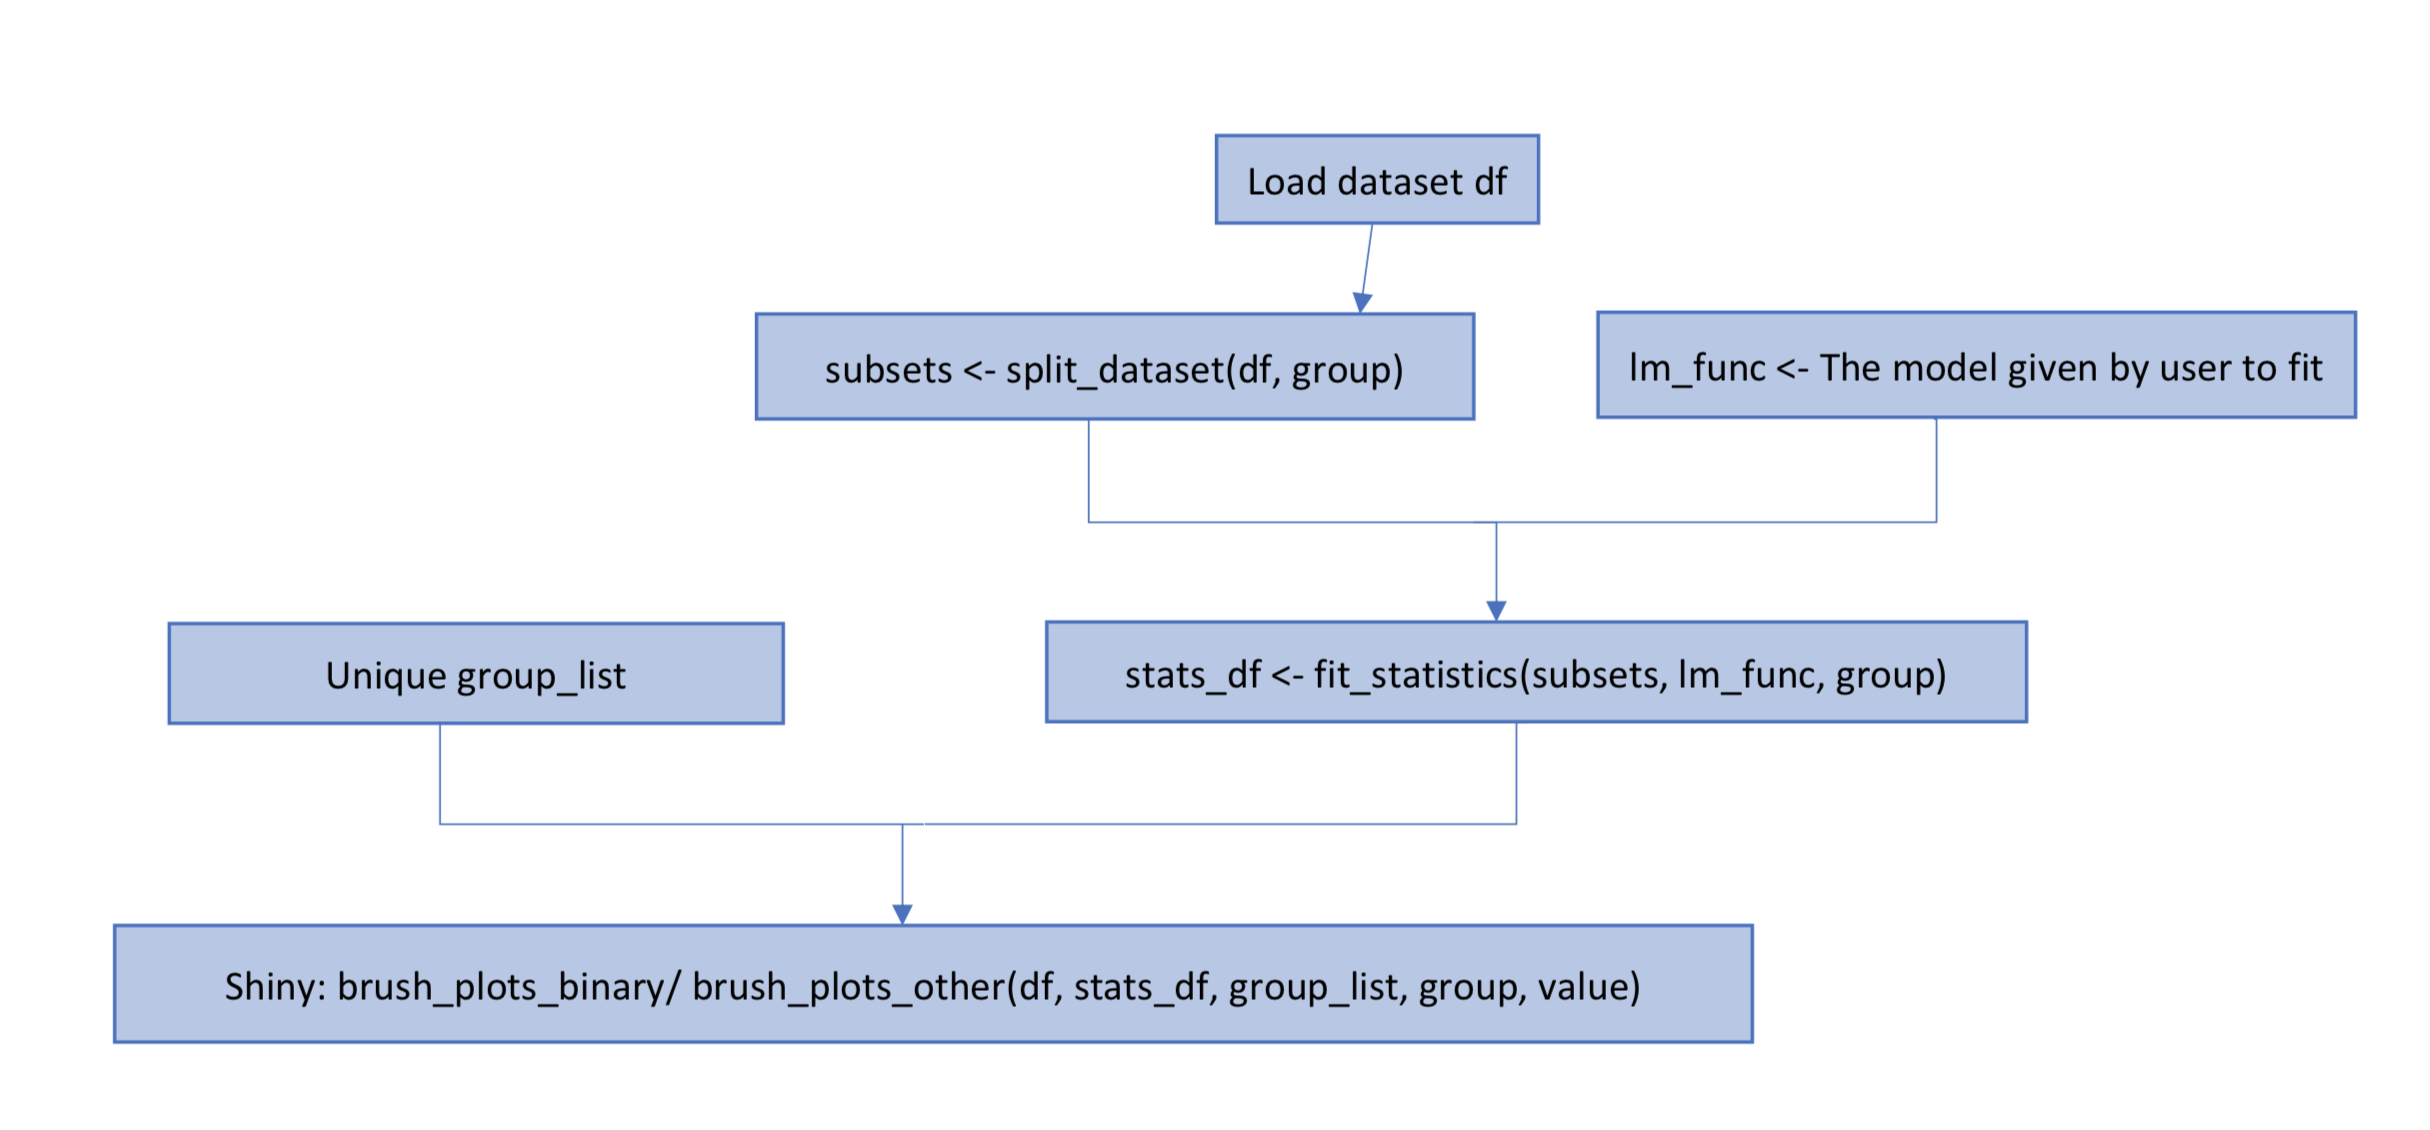
\includegraphics[width=400px]{../../MTBrush/workflow_pic} \caption[The overall MTBrush workflow, including helper functions for deriving multiple hypothesis test statistics and final visualization]{The overall MTBrush workflow, including helper functions for deriving multiple hypothesis test statistics and final visualization.}\label{fig:unnamed-chunk-5}
\end{figure}
\end{Schunk}

For example, for the randomly generated dataset above of binary
perturbations, we can launch the Shiny interface using the call below.

\color{violet}

I think it makes sense to include a visualization on the toy dataset.
But the table does not seem to be linked. Can you help debug this?

\begin{Schunk}
\begin{Sinput}
brush_plots_binary(example_data, fit_results, seq_len(1000), "feature", "estimate")
\end{Sinput}
\end{Schunk}

\color{black}

From this overview, users can interactively query for further details.
An example is given in Figure 3. This figures shows that, by brushing a
histogram, features lying in the mirrored range are highlighted in
orange; e.g., if the test statistic range \(t \geq 3\) was initially
selected, those with \(t \leq -3\) will appear in orange. Moreover,
features selected in one panel will be highlighted in the same color
across all histograms. This allows us to study the distribution of
statistics for all model terms within the selected set of features. In
particular, correlation across model terms will appear as high
significance simultaneously across several panels of histograms.

After the initial interaction, the original scatterplot from Figure 2B
will be replaced by the collection of scatterplots in D. Each panel in
this collection provides the measurements for one feature --- the 12
most significant features are shown by default, though more or less can
be included by modifying the ``ID'' dropdown menu (E). These
scatterplots of the original data support interpretation of test
results. For example, a large positive test statistic for a perturbation
may appear either because a feature is elevated in that perturbation or
because it is depressed in others -- the raw data can help disambiguate
these cases.

Finally, after brushing, a table (F) appears, providing contextual
information from the original input dataset associated with each
feature. The table also provides the exact test statistics and model
outputs, like estimated coefficients and \(p\)-values, associated with
each selected feature. Like the panels, the tables are sorted by the
magnitude of the test statistics, with the direction of effects color
coded to match the histograms. The table is paginated, and there is no
limit on the number of statistics that appear.

\begin{Schunk}
\begin{figure}
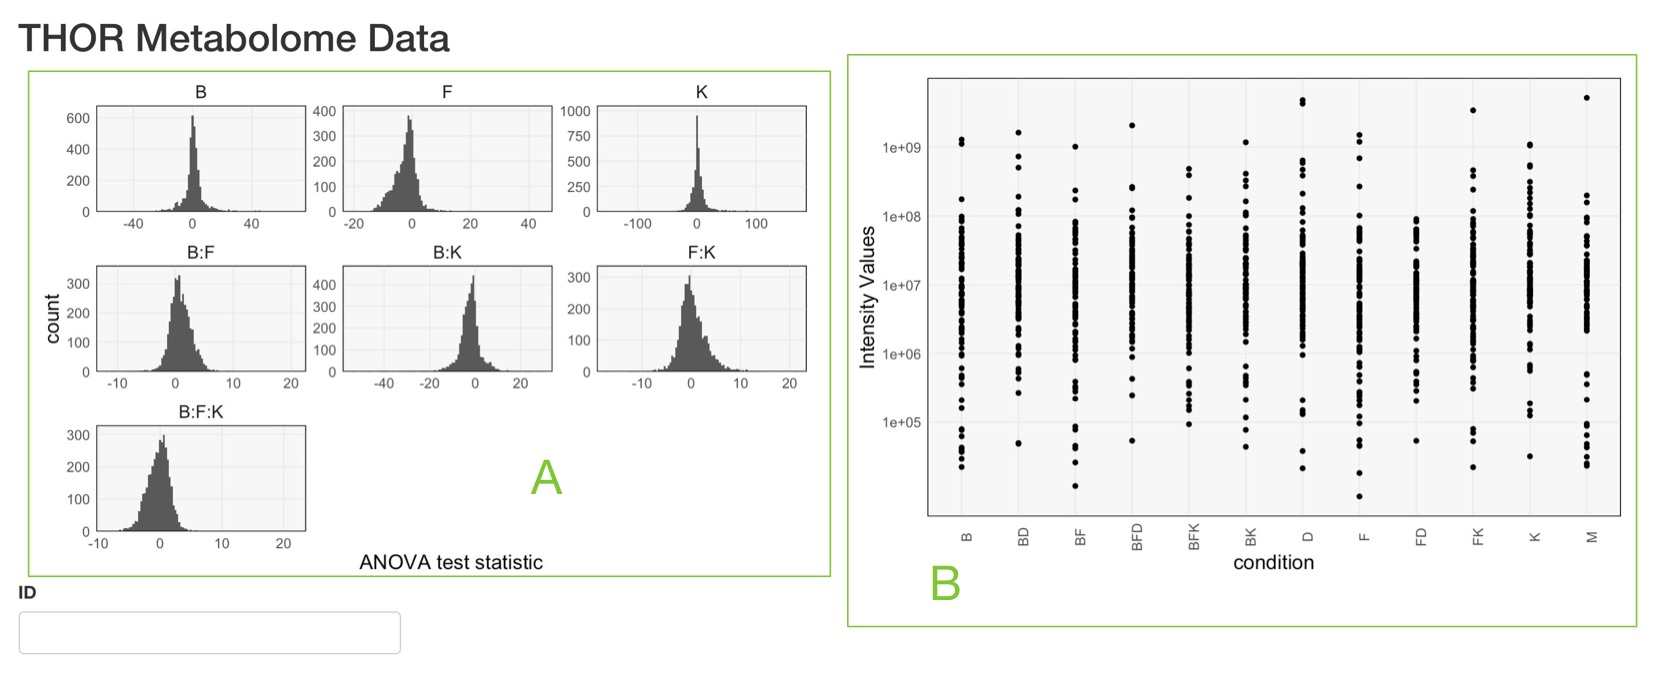
\includegraphics[width=400px]{../../MTBrush/interface1} \caption[Descriptions for each section of the initial interface]{Descriptions for each section of the initial interface. A: Histograms of test statistics, brush through any one of the histogram to select features;  B: Before brushing, a scatterplot of all features will appear to give an overall distribution of the dataset.}\label{fig:unnamed-chunk-7}
\end{figure}
\end{Schunk}

\color{purple}Is this information going to appear in the caption? If
not, we should think of how to transition to this description. Yes they
are the caption\color{black}

\begin{Schunk}
\begin{figure}
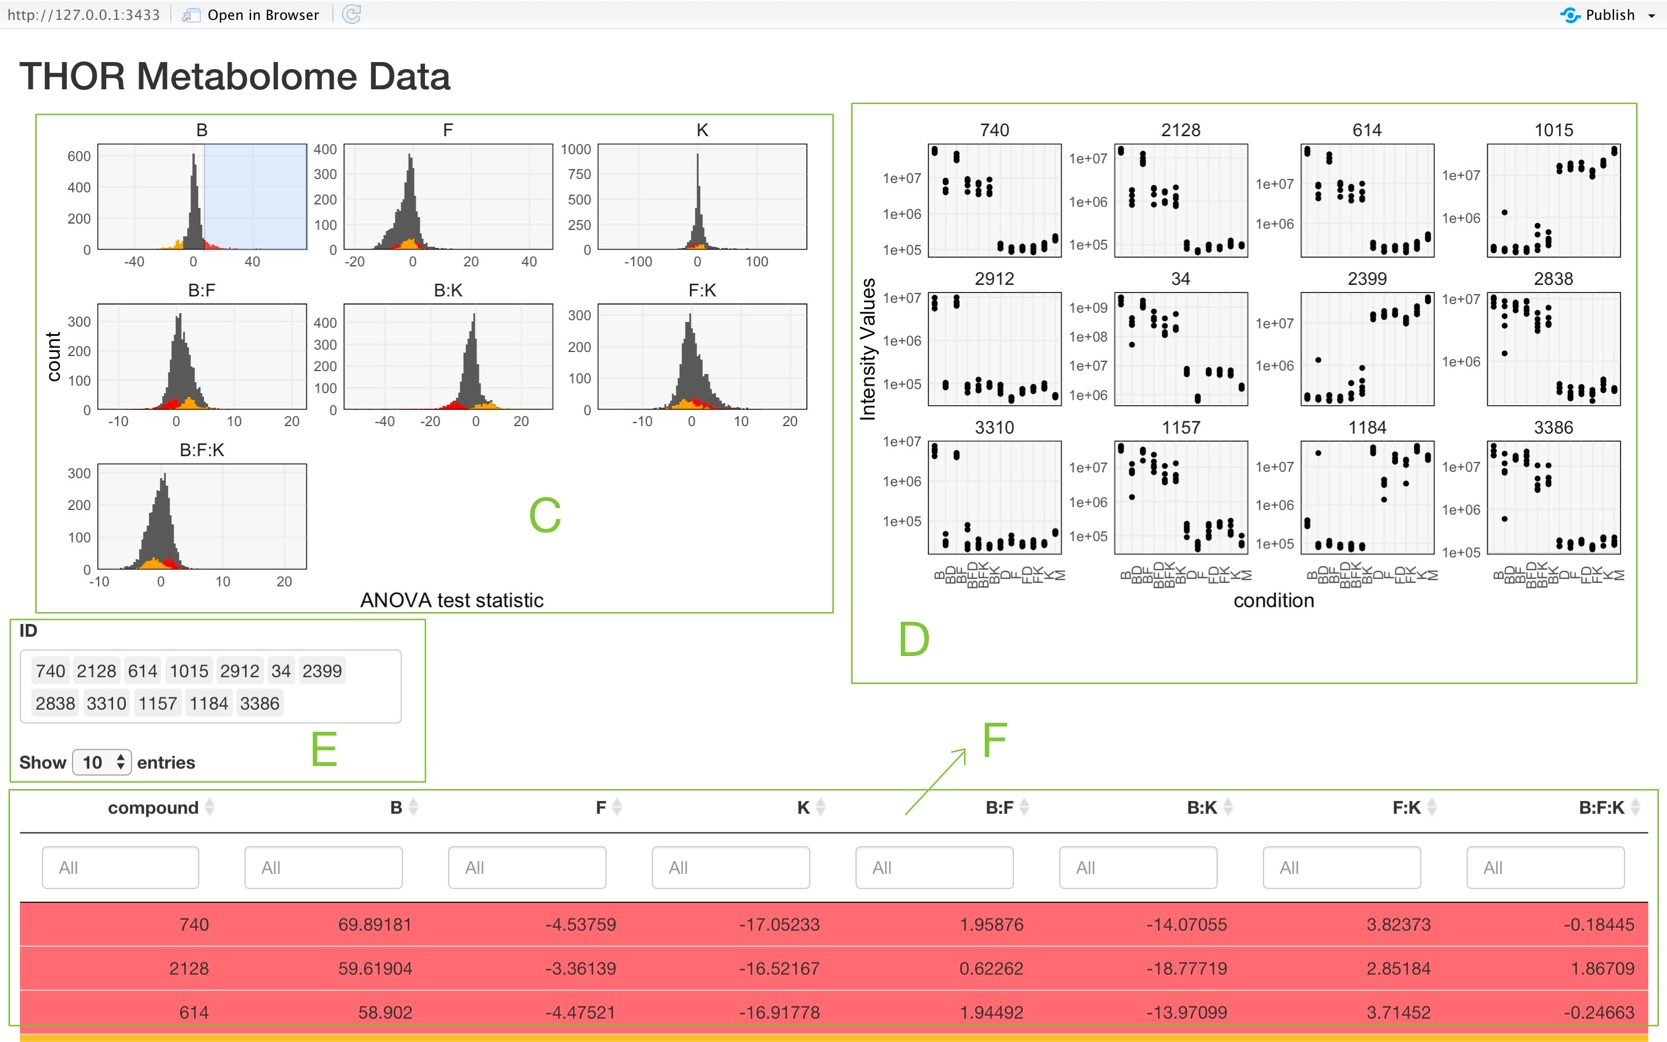
\includegraphics[width=400px]{../../MTBrush/interface2} \caption[Descriptions for each section of the interface after brushing]{Descriptions for each section of the interface after brushing. C: After brushing, test statistics with magnitude within the selected interval will be highlighted (red for selected and orange for reflected values). The selected features will be highlighted across all histograms; D: The scatterplots of top 12 features in the table of selected features will be shown here. By adding or deleting the chosen ID on the left select menu, users can choose to see the scatterplot of features of interest; E: By default, only 12 features will be chosen at first. Users can use the dropdown menu to follow the features of interest; F: The table of selected features in the brushed area. Colors match those in the upper histograms.}\label{fig:unnamed-chunk-8}
\end{figure}
\end{Schunk}

\hypertarget{cases-studies}{%
\section{Cases Studies}\label{cases-studies}}

We illustrate the use of the \texttt{MTBrush} package using two case
studies. Our examples are drawn from very different problem areas ---
metabolomic and spatial data analysis --- but share common sources of
complexity. Both problems require the application of regression models
in parallel across a large collection, producing test statistics across
both the terms in the model and members of the collection. It is
difficult to inspect results across both dimensions using raw model
output, and we illustrate how \texttt{MTBrush} can streamline the
process.

\hypertarget{discovering-interactions-in-a-model-microbial-system}{%
\subsection{Discovering interactions in a model microbial
system}\label{discovering-interactions-in-a-model-microbial-system}}

Our first case study considers metabolomic expression patterns in ``The
Hitchhicker's of the Rhizosphere'' (THOR) model microbial community
\color{violet}(cite Hurley, Chevrette)\color{black} designed to shed
light on the molecular biology of species interactions. Specifically,
this model system makes it possible to examine the microbial behaviors
that only emerge when multiple species are present in a shared
environment. A more systematic characterization of the mechanisms
through which microbes affect one another's behavior is a key first step
in the effort to design human-engineered microbial communities. Such
communities could be used to support human health and climate change
mitigation.

We consider data from this system from an experiment designed to
characterize the influence of species interactions on the community
metabolome. Specifically, 12 configurations of the THOR system were
grown, corresponding to the presence or absence of each of three
species, Bifidobacterium (todo?) (B), Flavobacterium johnsonii (F), and
either Pseudomonas Koreensis (K) or a corresponding mutant whose ability
to produce the antibiotic korreincene (todo?) has been knocked out
(Table X). Five replicates were gathered for each configuration, and
each was metabolically profiled using Liquid chromatography--mass
spectrometry (LCMS). The scientific goal of this study is to detect
compounds whose expression in joint communities (e.g., F + K) cannot be
explained by simply interpolating expression when each of the
constituent species are present in isolation. These metabolites may
reflect higher-level competitive or synergistic effects within the
community.

The code below loads the associated dataset, which contains 60 samples,
each with expression measurements across 3882 compounds.

\color{violet}

\begin{Schunk}
\begin{Sinput}
df <- read_csv("../../MTBrush/clean.csv") # Can you include the THOR dataset in the package by default? Or, if it is too large, create a link to directly download this dataset?
\end{Sinput}
\end{Schunk}

\color{black}

We frame the analysis as a parallel multiple hypothesis testing problem.
For each compound, we fit the saturated linear model
\texttt{log(Abundance)\ \textasciitilde{}\ B\ *\ F\ *\ K}. This is
captured by the \texttt{lm\_func} helper in the block below.

\begin{Schunk}
\begin{Sinput}
lm_func <- function(x) {
  lm(log(value) ~ B * F * K, data = x)
}

code <- function(z) { ifelse(str_detect(z, "\\+"), 1, -1) }
fits <- df %>%
  mutate(across(B:M, code)) %>%
  split_dataset(compound) %>%
  fit_statistics(lm_func, compound)
group_list <- unique(df$compound)
\end{Sinput}
\end{Schunk}

The main effects describe how the expression level for a compound varies
when the associated species are present or absent from the community.
Interaction effects measure the extent to which these effects are
modulated by coexistence of multiple species. For example, a strong,
positive \texttt{F\ :\ K} interaction terms for a compound suggests
that, in the FK condition, the compound is present at much higher levels
than would be expected when only one of F or K are present in isolation.

We launch our interface using the following call,

\begin{Schunk}
\begin{Sinput}
brush_plots_binary(df, fits, group_list, "compound", "value")
\end{Sinput}
\end{Schunk}

Figure \texttt{\textbackslash{}ref\{fig:thor\_overview\}} provides a
static overview of the interface before the user has provided any query.
From the scatterplot, we observe that the distribution of data points is
relatively uniform across conditions and there are no extreme outliers.

\begin{Schunk}
\begin{figure}
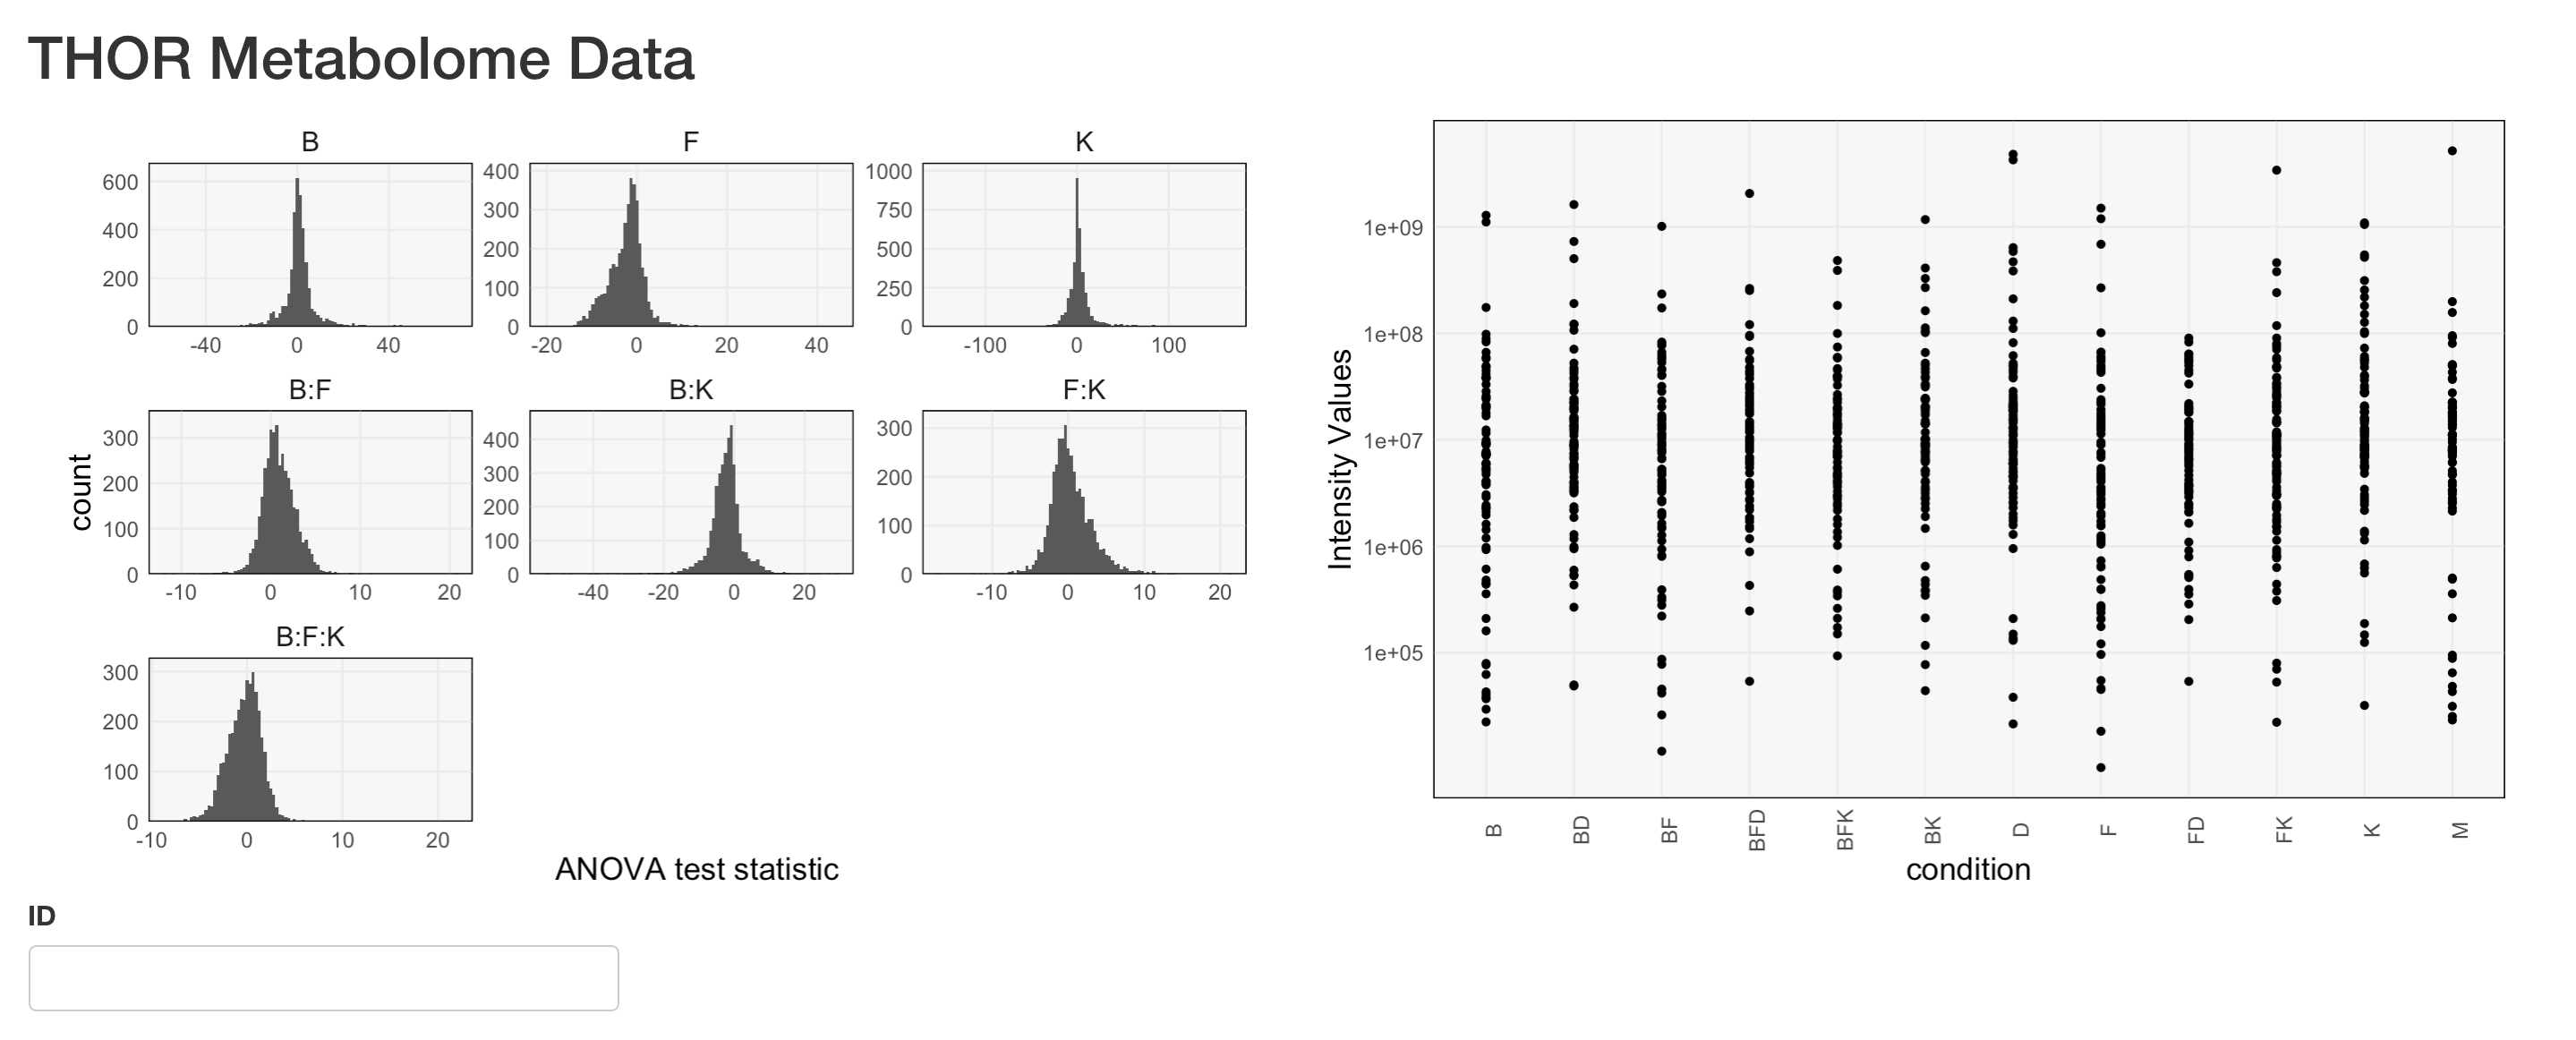
\includegraphics[width=400px]{../../MTBrush/before} \caption[The initial interface of the THOR data before interaction]{The initial interface of the THOR data before interaction}\label{fig:unnamed-chunk-12}
\end{figure}
\end{Schunk}

In the figure below, we brushed compounds with large, positive F
effects. In this selection, the associated FK effects are mostly
positive and the associated BFK effects are mostly negative -- compare
the orange bulk within this panel with 0. A possible explanation is that
these selected, orange compounds are consumed by F, which is why they
decrease in the presence of F. The positive FK effects suggest that
these compounds are not being consumed as rapidly when K is present.
This is consistent with a decrease in F's population induced by K's
production of the antibiotic koreenceine. Finally, considering the B:F:K
panel shows that these effects are generally negative. Therefore, the
high abundance F metabolites have a lower abundance than would be
predicted by a two-way interaction model alone. This is consistent with
B protecting F in the community, a previously documented phenomenon.

\begin{Schunk}
\begin{figure}
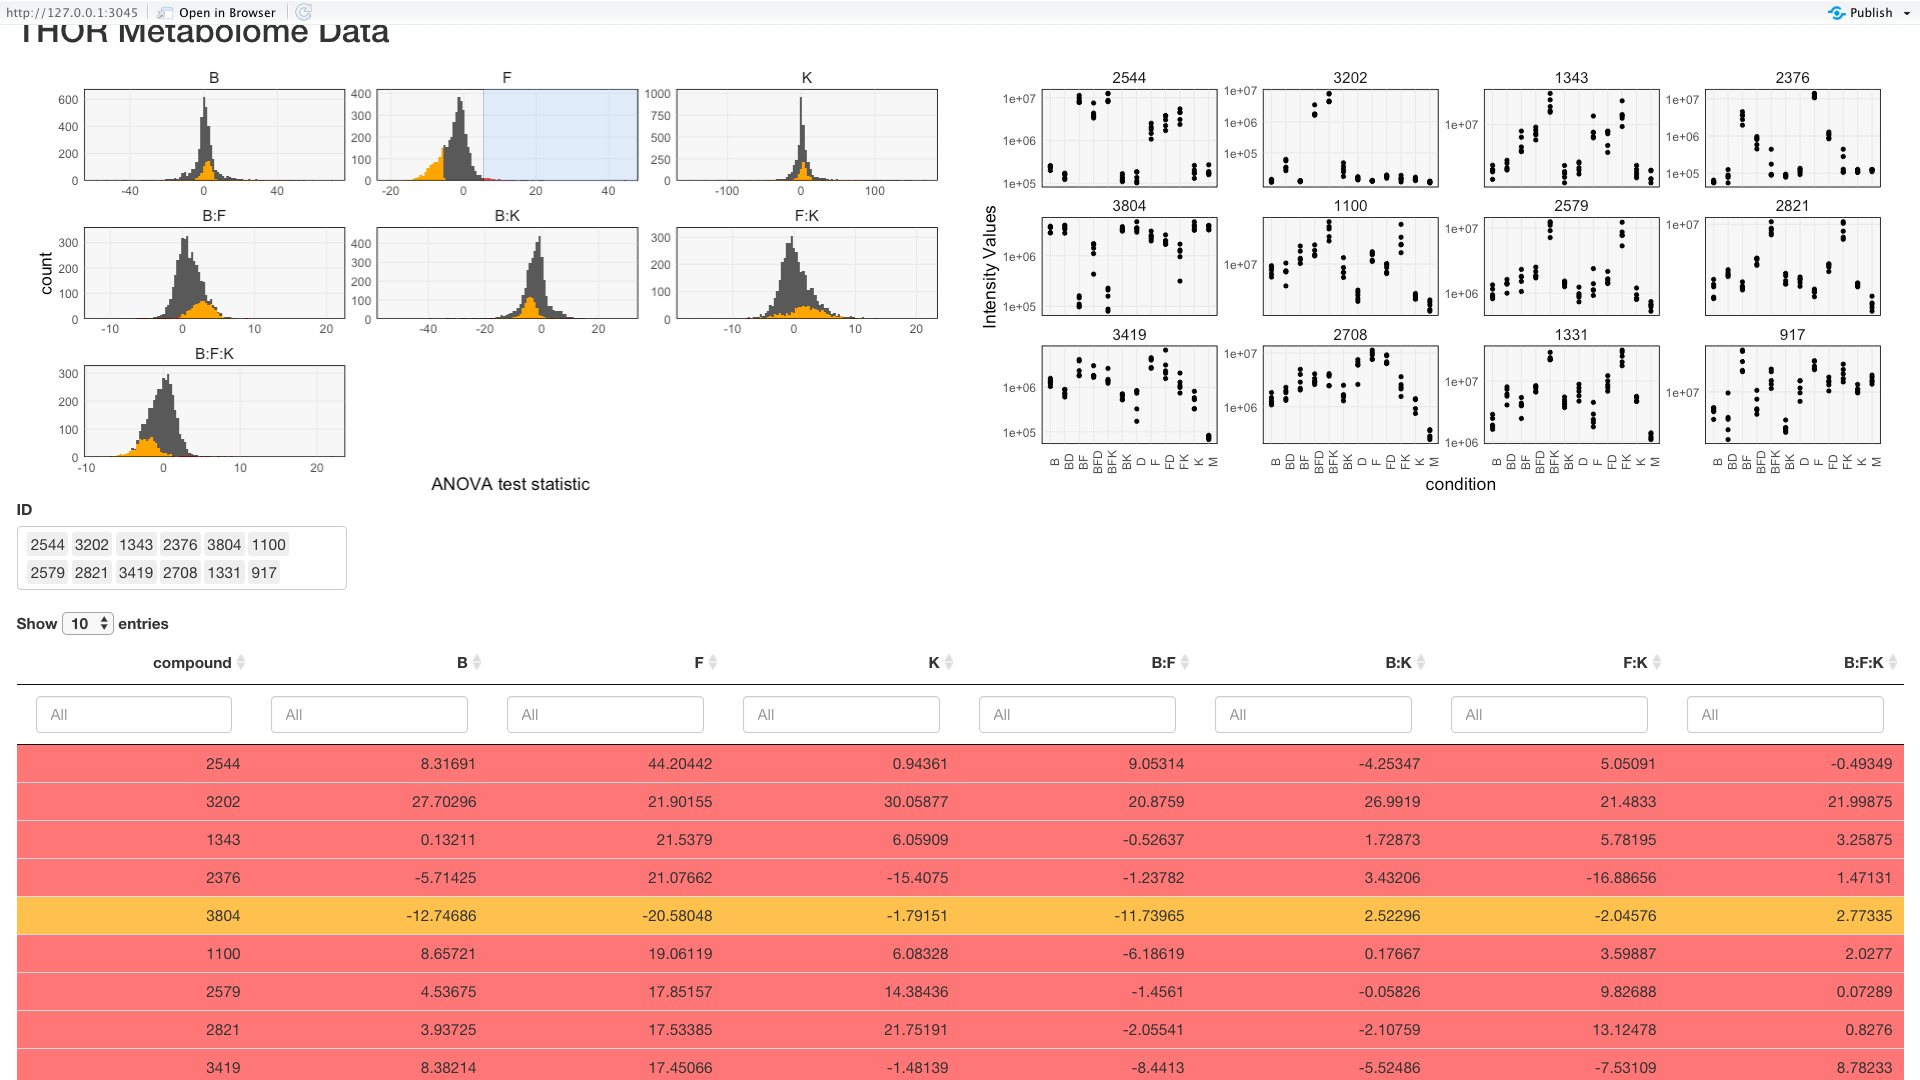
\includegraphics[width=400px]{../../MTBrush/Thor_example} \caption[The interface after brushing through compounds on the left tail of the F histogram]{The interface after brushing through compounds on the left tail of the F histogram}\label{fig:unnamed-chunk-13}
\end{figure}
\end{Schunk}

\hypertarget{navigating-california-home-prices}{%
\subsection{Navigating California home
prices}\label{navigating-california-home-prices}}

Our second example uses MTBrush to support exploration of the California
Housing Price dataset \cite{housing}. This dataset includes prices of
20,640 homes, together with features of the homes and their
neighborhoods, including the number of rooms and neighborhood's median
income, for example. The data are loaded in the block below,

\color{violet}

Can we also include the housing dataset in the package by default? Also,
can we include better names than \texttt{df\_old} and \texttt{df}?
\color{black}

These data are often used to evaluate supervised learning methods. Our
focus instead is to visualize how the conditions of a home and
neighborhood relate to observed prices, and how these effects vary
geographically. To understand how the influence of home and neighborhood
features are modulated by geographic location, we partition the dataset
into geographically disjoint sets and fit a linear model within each.
The coefficients from these models can be plotted as histograms and
brushed to identify features that are important in some locations but
not others. Since some locations have many more houses than others,
partitioning the data with a simple geographic grid would result in
highly imbalanced sample sizes across the ensemble. For areas with few
houses, the results would not be comparable to those in areas with
larger sample sizes. To address this, we first apply \(K\)-means to the
geographic coordinates of the observed homes, resulting in 2064 clusters
with more balanced sample sizes.

\begin{Schunk}
\begin{Sinput}
house_cluster <- house_price %>%
  select(longitude, latitude) %>%
  kmeans(2064)

house_balanced <- cbind(cluster = house_cluster$cluster, house_price) %>%
   group_by(cluster) %>%
   filter(n() > 10)
\end{Sinput}
\end{Schunk}

We compute test statistics and launch our app in the block below,

\begin{Schunk}
\begin{Sinput}
lm_func <- function(x) {
  lm(median_house_value ~ population * households * median_income, data = x)
}

subsets <- split_dataset(house_balanced, cluster)
fits <- fit_statistics(subsets, lm_func, cluster)
group_list <- unique(house_balanced$cluster)
brush_plots_nonbi(house_balanced, fits, group_list, cluster, median_house_value)
\end{Sinput}
\end{Schunk}

Figure \ref{fig:homestart} shows the distribution of variable features
before any user interactions. From this overview, we notice that the
home prices are inversely related to the population density. In Figure
\ref{fig:homebrush}, we brushed to highlight those houses with positive
households effects. We find that the corresponding households and median
income interaction effects are negative, suggesting that median income
restrains the positive effects of households. Specifically, an increase
in the median income of a neighborhood has a smaller effect on average
home price when the number of households in that neighborhood is large.
When the population variable is also added, the three-way interaction
term seems to have a positive effects again.

For this dataset, it is typical to fit a single nonlinear model use it
to make predictions for house price. Interpreting the result of this fit
can be challenging, however. In contrast, by interacting with a full
ensemble of simple models, we can easily compare geographic variation in
effects, using individual panels to observe characteristics of
individual homes in each area.

\begin{Schunk}
\begin{figure}
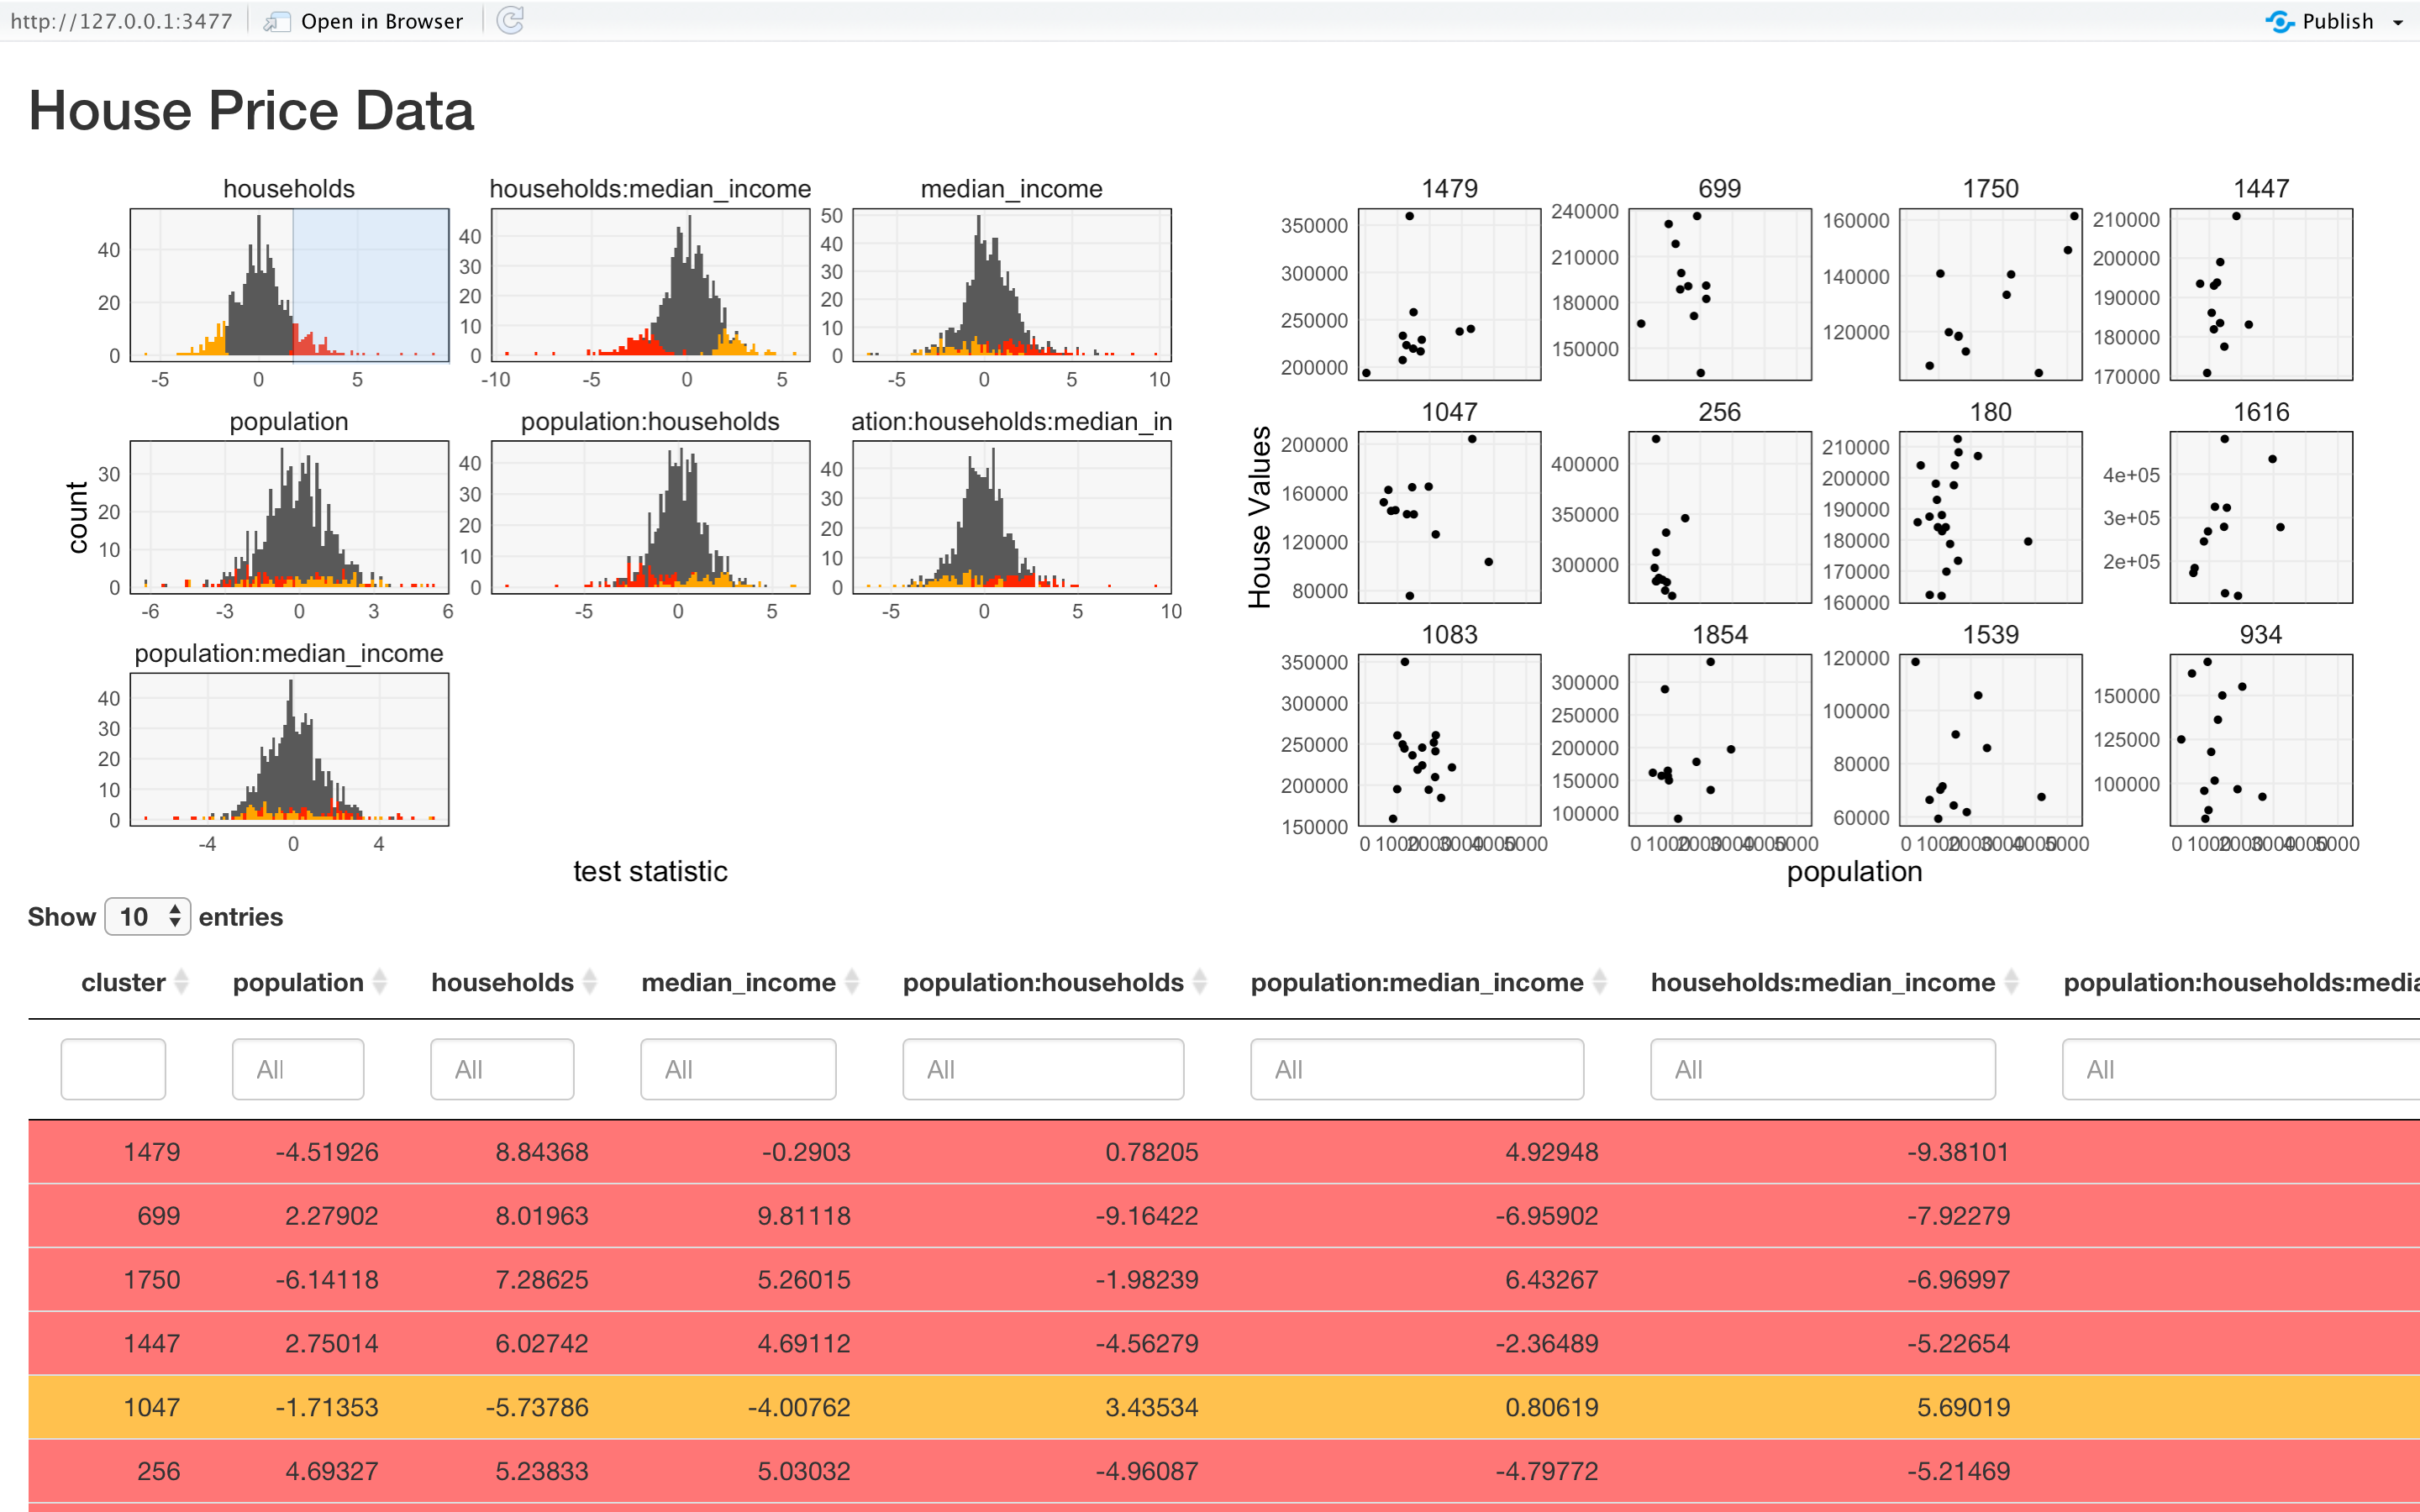
\includegraphics[width=400px]{../../MTBrush/example2} \caption[The interface after selecting houses with positive households effects in the house price example]{The interface after selecting houses with positive households effects in the house price example}\label{fig:unnamed-chunk-17}
\end{figure}
\end{Schunk}

\hypertarget{summary}{%
\section{Summary}\label{summary}}

MTBrush supports interactive visualization of multiple hypothesis
testing results. It is especially suited to settings where several test
statistics are extracted per feature; for example, when a multiple
regression model is fitted across features. The package provides
functions to guide data preparation, model fitting, and final
interactive visualization. We have found the package effective in
perturbation experiments (case study 1), though it can be applied to
understand the relationship between main and interaction effects in
multiple testing scenarios more generally (case study 2). We find that
brushing through linked views provides an intuitive and efficient
approach to exploring multiple hypotheses.

Though the provided helpers allow user to specify arbitrary test
statistics within each feature, we do not yet supply diagnostics for
checking model fit or validity. We also do not report local false
discovery rate estimates associated with selected test statistics. It
would be worthwhile to develop a brushing function for datasets of mixed
types, since the package in its current form only applies to homogeneous
binary or continuous inputs. These are all areas for future development.
Finally, though the path is less clear, we note that recent work has
suggested the possibility of accounting for interactive exploration of
hypotheses in simple setups \color{violet}{[}cite Lei and
Fithian{]}\color{black}, and integrating this work into the MTBrush
interface is an intriguing possibility.

The MTBrush package can be installed by running
\texttt{remotes::install\_github("YixingTT/MTBrush/MTBrush")} Detailed
documentation can be found at \url{tinyurl/link}. The interactive
interfaces created in our case studies can be viewed by visiting
\url{first/shiny/demo} and \url{second/shiny/demo}.

\bibliography{MTBrush-R-Journal.bib}

\address{%
Yixing Tu\\
University of Wisconsin-Madison\\%
1300 University Ave\\ Madison, WI\\ 53706\\
%
%
\textit{ORCiD: \href{https://orcid.org/0000-0002-9079-593X}{0000-0002-9079-593X}}\\%
\href{mailto:ytu26@wisc.edu}{\nolinkurl{ytu26@wisc.edu}}%
}

\address{%
Marc Chevrette\\
\\%
\\
%
%
%
%
}

\address{%
Chris Thomas\\
\\%
\\
%
%
%
%
}

\address{%
Jo Handelsman\\
\\%
\\
%
%
%
%
}

\address{%
Kris Sankaran\\
University of Wisconsin-Madison\\%
1300 University Ave\\ Madison, WI\\ 53706\\
%
\url{https://krisrs1128.github.io/LSLab}\\%
\textit{ORCiD: \href{https://orcid.org/0000-0002-9079-593X}{0000-0002-9079-593X}}\\%
\href{mailto:ksankaran@wisc.edu}{\nolinkurl{ksankaran@wisc.edu}}%
}
